%%%%%%%%%%%%%%%%%%%%%%%%%%%%%%%%%%%%%%%%%
% Twenty Seconds Resume/CV
% LaTeX Template
% Version 1.0 (14/7/16)
%
% Original author:
% Carmine Spagnuolo (cspagnuolo@unisa.it) with major modifications by 
% Vel (vel@LaTeXTemplates.com) and Harsh (harsh.gadgil@gmail.com)
%
% License:
% The MIT License (see included LICENSE file)
%
%%%%%%%%%%%%%%%%%%%%%%%%%%%%%%%%%%%%%%%%%

%----------------------------------------------------------------------------------------
%	PACKAGES AND OTHER DOCUMENT CONFIGURATIONS
%----------------------------------------------------------------------------------------

\documentclass[a4paper,14pt]{twentysecondcv} % a4paper for A4

% Command for printing skill overview bubbles
\newcommand\skills{ 
~
	\smartdiagram[bubble diagram]{
        \textbf{~~~~Full Stack~~~~}\\\textbf{Web Dev},
        \textbf{~~~~~OOP~~~~~~},
        \textbf{Interpersonal}\\\textbf{Skills},
        \textbf{Design},
        \textbf{Machine}\\\textbf{Learning},
        \textbf{Test}\\\textbf{~Automation~}
    }
}

% Programming skill bars
\programming{{Java $\textbullet$ Octave $\textbullet$ C $\textbullet$ C++ $\textbullet$ \large \LaTeX /},{SQL(MySQL) $\textbullet$ NoSQL(MongoDB)},{Python $\textbullet$ JavaScript $\textbullet$ HTML5 $\textbullet$ CSS3}}

\technologies{{Flask $\textbullet$ Django $\textbullet$ Selenium}}

\designskills{{Phototshop $\textbullet$ AutoCAD $\textbullet$ SolidWorks}}

% Projects text

%----------------------------------------------------------------------------------------
%	 PERSONAL INFORMATION
%----------------------------------------------------------------------------------------
% If you don't need one or more of the below, just remove the content leaving the command, e.g. \cvnumberphone{}
\cvpic{
	\begin{tikzpicture}
		\begin{scope}
			\clip [rounded corners=1.65cm] (0,0) rectangle coordinate (centerpoint) (3.3,3.3cm);
        	\node [inner sep=10pt] at (centerpoint) {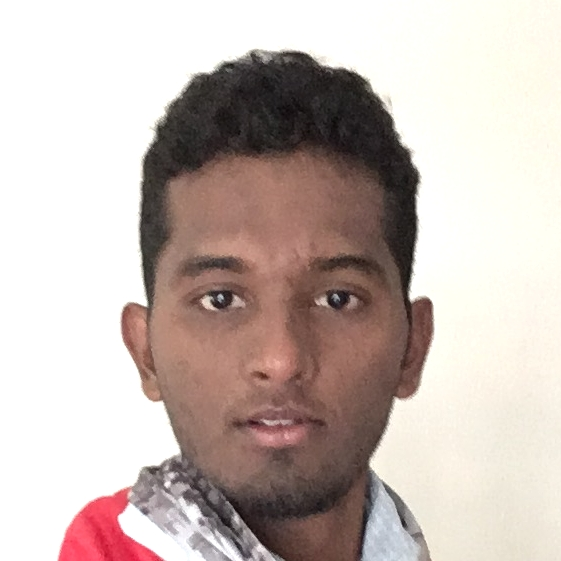
\includegraphics[width=3.3cm, height=3.3cm]{img/profile_2.JPG}};
		\end{scope}
	\end{tikzpicture}
}
\cvname{Vishnu Raveendran}% Your name
\cvjobtitle{ Software Engineer } % Job
\cvlinkedin{linkedin.com/in/vishnu-rvn}
\cvgithub{github.com/vishnu-rvn}
\cvnumberphone{Mobile: 9037 435 628} % Phone number
% \cvsite{hgadgil.com} % Personal website
\cvmail{Email: vishnunilambur@gmail.com} % Email address

%----------------------------------------------------------------------------------------

\begin{document}

\makeprofile % Print the sidebar

\section{Summary}
\vspace{4px}
\large
\begin{spacing}{1.2}
A hobbyist coder, designer, tester and an enthusiastic and quick learner looking to delve deep into the world of development as a full-stack developer specialized in python, equipped with good communication, logical and analytical skills. I am good at Python, getting better at HTML, CSS, Javascript, Java, web-development using Flask, and a beginner in Database technologies and Machine learning. I am looking forward to take on challenges in a quick-paced environment and effectively contribute to the growth of an organization.
\end{spacing}
%----------------------------------------------------------------------------------------
%	 EXPERIENCE
%----------------------------------------------------------------------------------------
\section{Experience}
\vspace{4px}

\begin{twenty} % Environment for a list with descriptions
\twentyitem
    	{\href{https://www.accenture.com/in-en}{Accenture}}
		{Sept 2017-Present}
        {Application Development Associate}
        {}
        {}
        {
        \begin{spacing}{1.2}                
        \begin{itemize}
        \item Currently working in life sciences industry. Involved in building interdependent modular applications, integration and customization of the same to suit the requirements of different pharmaceutical companies. Which are in turn used by them to accelerate their Research and Development processes. To reduce the cost and time involved in development of a drug.
        \item Maintain, refactor \& update automation frameworks built in Python and Java using selenium webdriver.
        \item Author, maintain \& execute automation and manual test scripts.
        \item Analyze and document defects in the defect documentation tool encountered during test executions.
        \item \textbf{Tools Used}: Rational Quality Manager, Rational Team Concert, Selenium, Python, Java
        \end{itemize}
        \end{spacing}}
        \\
        
	%\twentyitem{<dates>}{<title>}{<location>}{<description>}
\end{twenty}


\section{Personal Projects}
\vspace{4px}

\begin{spacing}{1.2}
\large
\textbf{Analytica} - Analytics application being built for data processing and visualization. Being built to focus on improving the understanding of AJAX using Javascript. Tools used: Flask, Python, Javascript, HTML, CSS, MongoDB\\
\textbf{Medium} - A mini blog website. Built primarily to focus on enhancing back-end and front-end programming. Tools used: Flask, Python, Javascript, HTML, CSS, MySQL\\
\textbf{Ecommerce} - An e-commerce website. Built primarily to focus on enhancing programming skills and to familiarize the concept of pagination(limit-offset method). Tools used: Flask, Python, Javascript, HTML, SCSS, MongoDB\\
\end{spacing}

%----------------------------------------------------------------------------------------
%	 EDUCATION
%----------------------------------------------------------------------------------------

\pagebreak
\makeprofiletwo

\vspace*{5mm}
\section{Education}

\begin{twenty} % Environment for a list with descriptions
	\twentyitem
		{{Government Engineering College, Thrissur}}
    	{August 2013 - May 2017}
        {B.Tech, Mechanical Engineering\textnormal{(GPA: 7.27/10.0)}}
        {}
        {}
        {}
	%\twentyitem{<dates>}{<title>}{<organization>}{<location>}{<description>}
\end{twenty}

\large{\textcolor{black}{Certifications}}
\vspace{4px}

\begin{twentyshort}
	\twentyitemshort
		{}
		{Intro to Python for Data Science}
		{\textbf{DataCamp}}
	\twentyitemshort
		{}
		{Intro to SQL for Data Science}
		{\textbf{DataCamp}}
	\twentyitemshort
		{}
		{Introduction to Python for Data Science (edX)}
		{\textbf{edX}}
	\twentyitemshort
		{}
		{Regex Academy: An Introduction To Text Parsing Sorcery}
		{\textbf{Udemy}}
	\twentyitemshort
		{}
		{Python for Data Science and Machine Learning Bootcamp}
		{\textbf{Udemy}}
\end{twentyshort}

\section{Other Interests}
\vspace{4px}

\begin{twenty}
Coding, Mountaineering \& hiking, gaming, books
\end{twenty}

\end{document} 